\begin{frame}
	\frametitle{Neutronics Results}
		\begin{columns}
			\column{5cm}
				\textbf{Serpent Input Parameters}
					\begin{itemize}
						\item Neutron population
							\begin{itemize}
								\item 200,000 neutrons per cycle
								\item 50 inactive, 500 active cycles
								\item 5 pcm statistical error in $k_{eff}$
							\end{itemize}
						\item JEFF-3.1.2 nuclear data library
						\item Six neutron energy groups
						\item Eight delayed neutron precursor groups
						\item Temperatures defined from 900 K to 1200 K at 50 K
						intervals
					\end{itemize}
			\column{5.5cm}
				\begin{figure}
					\centering
					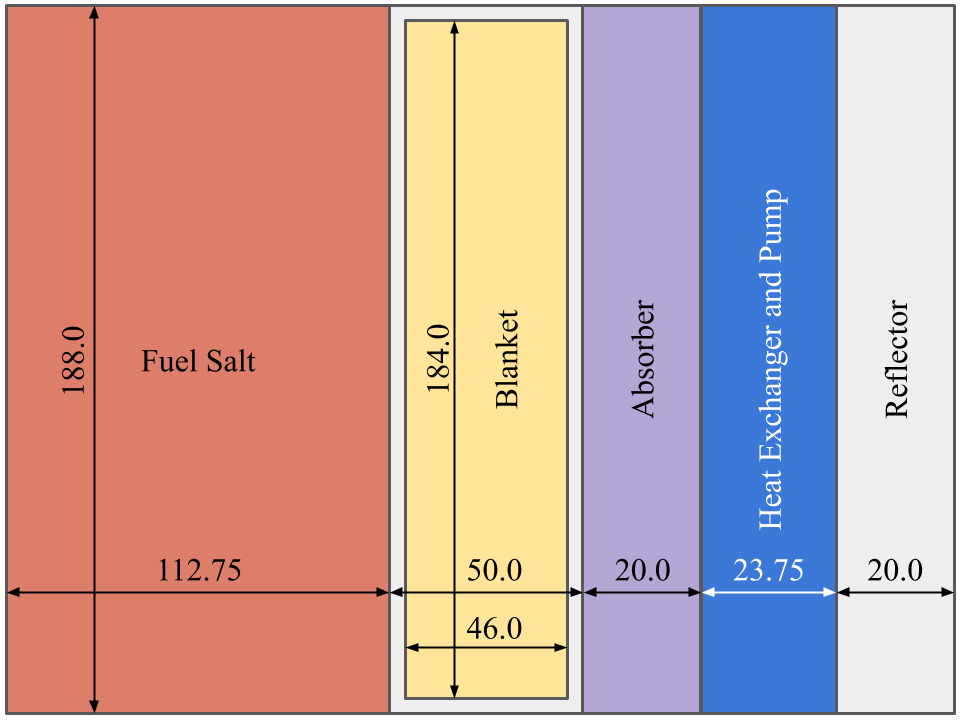
\includegraphics[width=\textwidth]
					{./images/reference}
					\caption{2D axisymmetric model used in Serpent. Derived from
					the \gls{MSFR} reference model
					\cite{fiorina_modelling_2014}. (Figure not to scale)}
					\label{fig:reference}
				\end{figure}
		\end{columns}
\end{frame}

\begin{frame}
	\frametitle{Neutronics Results}
		\textbf{Fuel Composition Data}
			\begin{itemize}
				\item Depletion calculations performed in a previous paper by
				A. Rykhlevskii, B. Betzler, A. Worrall, and K. Huff
				\cite{rykhlevskii_fuel_2019}
				\item 60-year depletion calculation on SCALE/TRITON
				using a unit cell representation of the \gls{MSFR}
				\item U/Th breeder reprocessing scheme
				\begin{itemize}
					\item Th feed, with some $^{233}$U from the blanket rerouted
					to the fuel salt to maintain criticality
				\end{itemize}
				\item Compositions:
				\begin{itemize}
					\item Start-up: LiF - ThF$_4$
					- UF$_4$ (77.5\% - 19.9\% - 2.6\%)
					\item Early-life: 300 days after start-up
					\item Equilibrium: 43 years after start-up
					($<$3\% change in TRU vector between depletion
					time-steps)
				\end{itemize}
			\end{itemize}
\end{frame}

\begin{frame}
	\frametitle{Neutronics Results}
	\begin{columns}
		\column{5.5cm}
		\textbf{Moltres Simulation Details}
		\begin{itemize}
			\small
			\item Adaptive backward Euler time-stepper
			\item Six neutron groups
			\item Eight \gls{DNP} groups
			\item Vacuum neutron boundary condition on outer edges
			\item Uniform upward flow of 1.125 m s$^{-1}$
			\item Flow/decay of \glspl{DNP} and heat removal in the outer loop
			is simulated on a simplified 1D geometry separate from active core
			region
			\item Fixed heat removal rate, $Q_{hx}$, to secondary loop system
		\end{itemize}
		\column{5cm}
		\begin{figure}
			\centering
			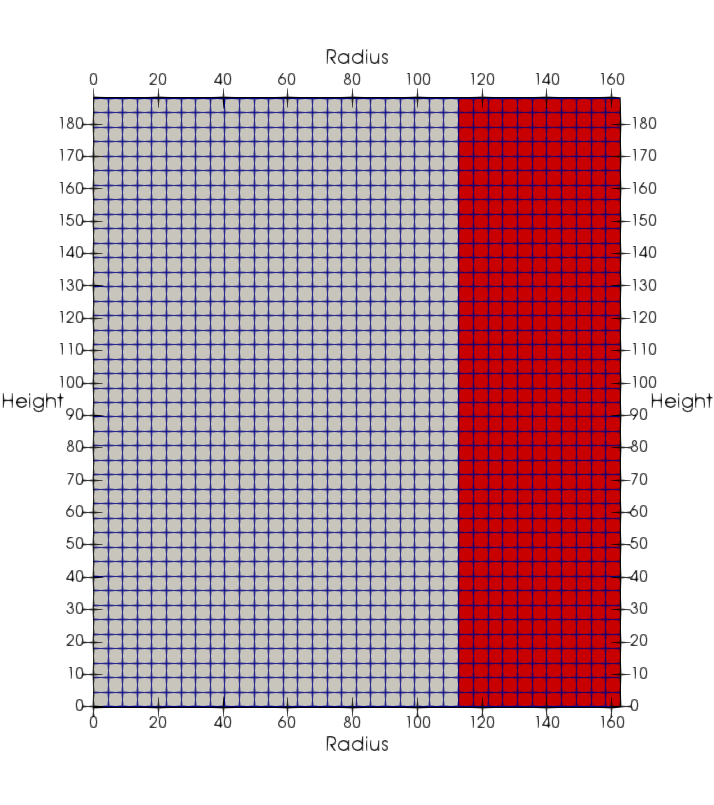
\includegraphics[width=\textwidth]{./images/mesh}
			\caption{\footnotesize Mesh of the 2D axisymmetric model used in
			Moltres. The
			grey and red regions represent the fuel and blanket salt
			respectively.}
			\label{fig:mesh}
		\end{figure}
	\end{columns}
\end{frame}

\begin{frame}
	\frametitle{Neutronics Results}
		\textbf{Results}
			\begin{figure}
				\centering
				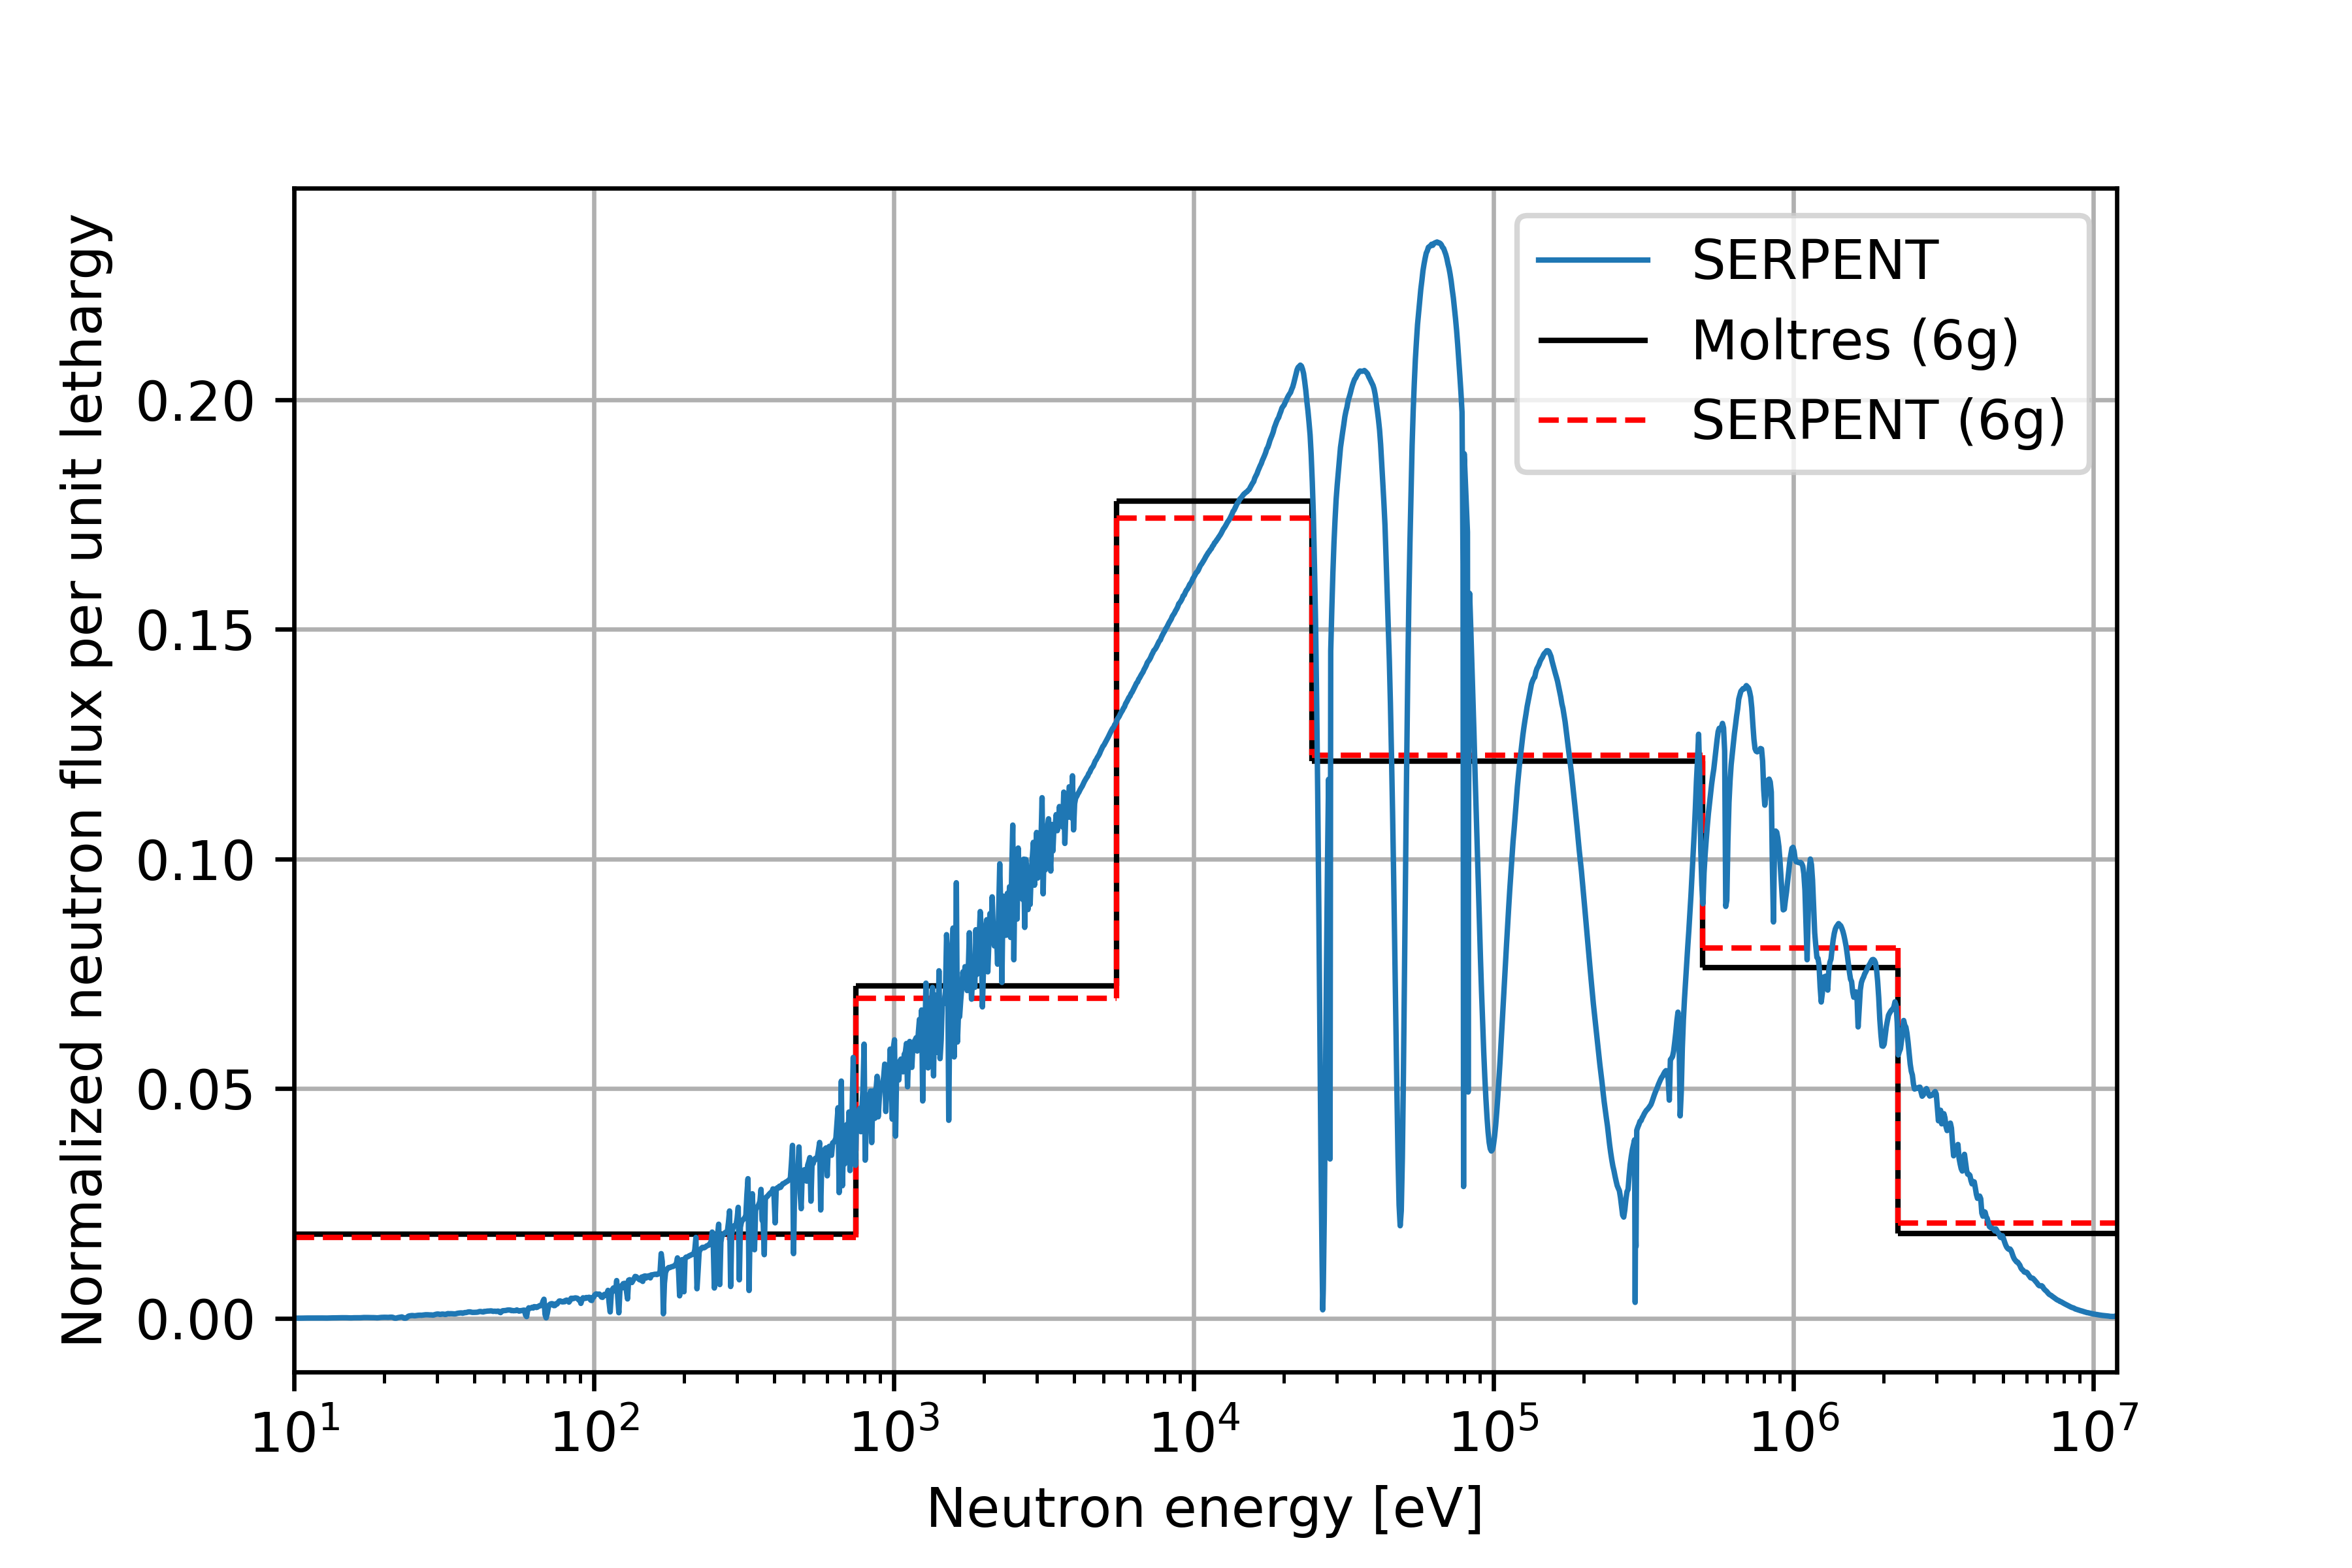
\includegraphics[width=.8\textwidth]{../paper/figures/nt-spec}
				\caption{Continuous and six energy group neutron flux
				distributions from Serpent and Moltres (start-up composition
				without \gls{DNP} drift at 973 K).}
				\label{fig:ntspec}
			\end{figure}
\end{frame}

\begin{frame}
	\frametitle{Neutronics Results}
		\textbf{Fuel Temperature Reactivity Feedback}
			\begin{table}[t]
				\centering
				\caption{Fuel temperature reactivity feedback coefficients with
				the start-up fuel composition.}
				\begin{tabular}{lccc}
					\hline
					\multirow{2}{*}{Composition} & {$\alpha_T$ [pcm K$^{-1}$]} & {$\alpha_T$ [pcm K$^{-1}$]} & Difference [\%]\\
					& Serpent & Moltres & \\
					\hline
					Start-up & $-7.39 \pm 0.03$ & $-7.46$ & $-0.94$\\
					Early-life & $-7.25 \pm 0.03$ & $-7.33$ & $-1.1$\\
					Equilibrium & $-6.24 \pm 0.03$ & $-6.34$ & $-1.6$\\
					\hline
				\end{tabular}
				\label{table:reactivity}
			\end{table}	
\end{frame}
